% ********** Chapter 4 **********
\chapter{AVL-boom}
\label{sec:Hoofdstuk 4}

\begin{figure}[h]
	\centering
		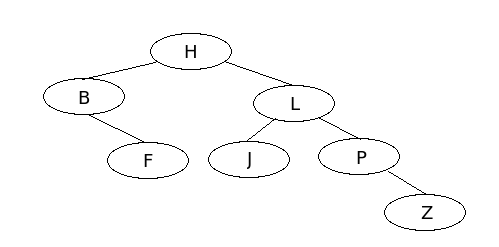
\includegraphics[width=\textwidth]{chap4/avltree}
	\label{fig:avltree}
\end{figure}

\section{Introductie}
De AVL-boom is de eerste gebalanceerde boom die we gaan behandelen. Deze boom lijkt erg veel op de binary boom, alleen heeft de AVL-boom een extra eigenschap, namelijk dat voor elke interne knoop geldt dat de hoogte van de kinderen verschilt met maximaal 1.\\
\\
\section{Zoeken}
Het zoeken gaat op dezelfde manier als bij de binaire boom die behandeld is in hoofdstuk 2.\\
\\
\section{Toevoegen}
Het toevoegen van nodes aan de AVL boom, werkt hetzelfde als bij een normale binaire boom. Maar nadat de node aan de boom is toegevoegd zal er gecontroleerd worden of de boom nog steeds aan zijn eigenschappen voldoet. Is dit niet het geval, dan zal er door middel van zo genaamde rotations de balans weer hersteld worden. Omdat dit na elke toevoeg actie gedaan wordt, zijn er maximaal twee rotations nodig om de hele boom weer in balans te krijgen.

% ********** End of chapter **********